Los criterios a evaluar fueron estimados con el rango de notas de 1 a 7, sacando un promedio de cada integrante del equipo según la percepción que obtuvo al utilizar el software: \\

\begin{center}
\begin{tabular}{|l|c|p{2.40in}|}
 \hline
 \textbf{Criterio} & \textbf{Nota} & \textbf{Comentario} \\
 \hline
 \textbf{Fácil de Implementar} & 7.0 & Es una herramienta 100\% web, por lo que no necesariamente el software necesita ser instalado en el computador. \\
 \hline
 \textbf{Facilidad de uso} & 5.0 & Presenta una interfaz poco intuitiva (Diseño Drag and Drop). \\
 \hline
 \textbf{Estándares} & 6.0 & No utiliza la misma notación de BPMN 2.0 pero son semejantes, su notación esta orientada a SOA (arquitectura orientada a servicios). \\
 \hline
 \textbf{Licencia} & 7.0 & ProcessMaker brinda a las organizaciones las ventajas de open source. \\
 \hline
 \textbf{Documentación y Soporte} & 7.0 & La página web del software presenta una gran variedad de documentación , vídeos y foros en que se enseña a utilizar el software, además posee un servicio de soporte. \\
 \hline
\end{tabular}
\end{center}

\subsection{Ejemplo de Proceso de obtención de tarjeta de crédito}
Para la utilización del software ProcessMaker, según el modelamiento de procesos, se utilizó como referencia un video de youtube que explicaba la obtención de una tarjeta de crédito en un banco.

También se pudo observar que este software posee la capacidad de que el administrador pueda interactuar con cualquier trabajador de la empresa en algún proceso, puesto que existe la opción de agregar usuarios, grupos o departamentos, en que el administrador puede asignarles tareas o sub-tareas, también poder enviarles reportes, mensajes (en el mismo software hay un inbox) o mails. Además esta la opción que si alguna tarea requiere de la creación de formularios, se realiza de forma dinámica, en el ejemplo de la tarjeta de crédito se requiere en la tarea de ``Rellenar Solicitud", un formulario en que se ingresen los datos del cliente y fecha en que se realizó la solicitud, entonces en esta tarea el usuario de la empresa asignado en esta tarea tendrá la misión de ingresar mediante este formulario los clientes que serán luego guardados en una base de datos del mismo software.
 
\begin{center}
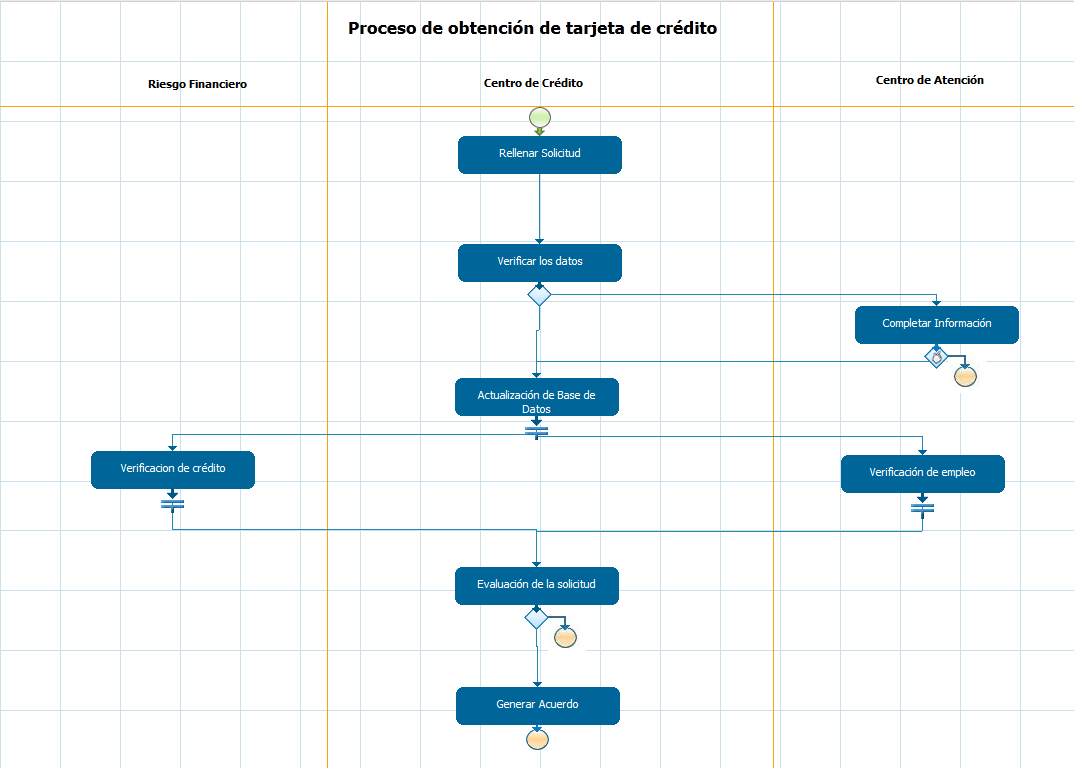
\includegraphics[scale=0.5]{./imagenes/modelos_pm.png}\\
     Figura 1: Modelo en Process Maker.\\
\end{center}

A continuación se muestra la notación del software:

%ingresar la notación